% Define the subtitle of the page
\title{Delving In}

% Begin the content of the page
\subsection{Delving In}

Edward enables black box inference for probability models. Its design reflects
the building blocks for inference and model criticism. Here we describe the
motivation behind Edward's design and specify its internal workings.

Edward is named after the innovative statistician
\href{https://en.wikipedia.org/wiki/George_E._P._Box}{George Edward
Pelham Box}. Edward follows Box's philosophy of statistics and machine
learning.

First gather data from a real-world process. Then cycle through Box's
loop:

\begin{enumerate}
\item Build a probabilistic model of the process
\item Reason about the process given model and data
\item Criticize the model, revise and repeat
\end{enumerate}

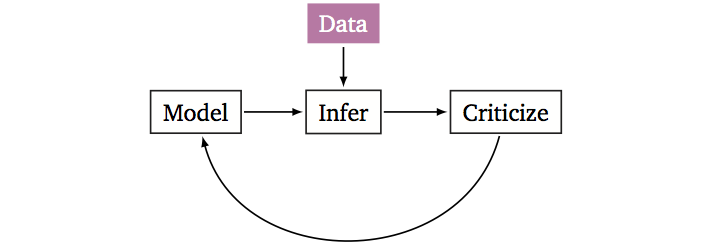
\includegraphics{images/model_infer_criticize.png}

Here's a toy example. A child flips a coin ten times, with the data of
outcomes being \texttt{{[}0,\ 1,\ 0,\ 0,\ 0,\ 0,\ 0,\ 0,\ 0,\ 1{]}}. We
are interested in the probability that the coin lands heads. First,
build a model: assume the coin flips are independent and land heads with
the same probability. Second, reason about the process: use an algorithm
to reason about the model given data. Third, criticize the model: analyze
whether the model captures the real-world process of coin flips. If it
doesn't, then revise the model and repeat.

This process defines the design of Edward. Four primary objects enable the
above analysis. 

\subsubsection{Data}

\texttt{Data} objects contain measurements. The structure of these objects must
match the inputs of the probabilistic model. For example, 

\begin{lstlisting}[language=Python]
data_np = np.array([0, 1, 0, 0, 0, 0, 0, 0, 0, 1])
my_data = ed.Data(tf.constant(data_np, dtype=tf.float32))
\end{lstlisting}

\texttt{Data} objects define a \texttt{sample} method that specifies how to
sample minibatches of observations from the dataset.

\subsubsection{Models}\label{models}

There are two types of model objects in Edward:
\begin{enumerate}
\item Probability models of data, $p(x,z)$
\item Variational models of latent variables $q(z\;;\;\lambda)$
\end{enumerate}

\textbf{Probability Models.}
Edward supports probability models specified in TensorFlow, NumPy/SciPy, PyMC3,
or Stan. A probability model has the following structure.
\begin{lstlisting}[language=Python]
import edward as ed
import tensorflow as tf

class probability_model():
    def __init__(...):
        ...
        self.num_vars = ...
 
    def log_prob(self, xs, zs):
        log_prior = ...
        log_likelihood = ...
        return log_prior + log_likelihood

my_model = probability_model(...)
\end{lstlisting}
The field \texttt{self.num\_vars} holds the number of latent variables in the
probability model. For example, a model with a Gaussian likelihood with latent
mean and variance would have \texttt{self.num\_vars=2*N} latent variables for 
\texttt{N} observations.

The method \texttt{self.log_prob(xs, zs)} calculates the log probability of the
joint density $\log p(x,z)$. Here \texttt{xs} contains the data and \texttt{zs}
are the latent variables.

This describes the probability model, which is a joint distribution of data $x$
and latent variables $z$. Given a model, we aim to reason about $z$ given some
data: the latent patterns conditioned on some data. The posterior distribution
$p(z \mid x)$ captures our reasoning: its mean describes our best guess of the
latent patterns, and its variance describes the uncertainty around our best
guess. 

\textbf{Variational Models.}
Edward uses variational inference to approximate the posterior. To this end,
Edward implements a foundational \texttt{Variational()} class and a library of
\texttt{Distribution()} objects. Variational models combine these using
the \texttt{add()} syntax.

For example, to specify this variational model (e.g.~for a Gaussian mixture)
\begin{align*}
  q(z \;;\; \lambda) 
  &=
  \text{Dirichlet}(z_\pi)
  \times
  \mathcal{N}(z_\mu)
  \times
  \text{LogNorm}(z_\sigma)
\end{align*}
we would write
\begin{lstlisting}[language=Python]
from edward.models import Variational, Dirichlet, Normal, LogNorm

my_variational = Variational()
my_variational.add(Dirichlet(K))
my_variational.add(Normal(K*D))
my_variational.add(LogNorm(K*D))
\end{lstlisting}
Ordering matters; variational models must match the same ordering as latent
variable declarations in \texttt{probability_model.log_prob(xs, zs)}.

\subsubsection{Inference}\label{inference}

Edward implements a variety of inference procedures. Current techniques
leverage variational inference, which seeks to match the variational model
$q(z \;;\; \lambda)$ to the posterior of the probability model 
$p(z \mid x)$.

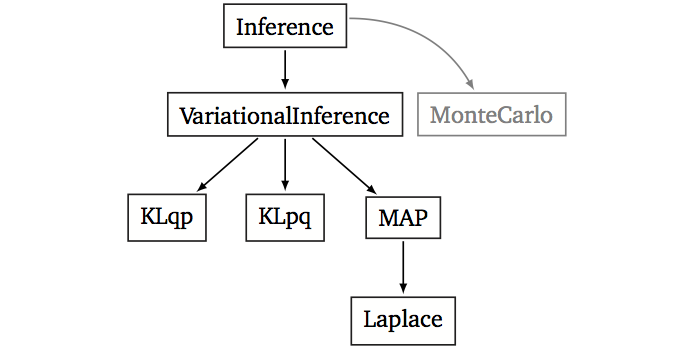
\includegraphics{images/inference_structure.png}

Each algorithm minimizes a different loss metric between the variational model
and the posterior. Algorithms that derive from \texttt{VariationalInference()}
take as input a probability model, a variational model, and data. 

For example, to minimize the Kullback-Leibler divergence
\begin{align*}
  \text{KL}(p(z \mid x) \;\|\; q(z \;;\; \lambda))
\end{align*}
we would write
\begin{lstlisting}[language=Python]
inference = ed.KLpq(my_model, my_variational, my_data)
inference.run(n_iter=500, n_minibatch=5)
\end{lstlisting}
which runs the \texttt{KLpq} minimization algorithm for \texttt{500} iterations,
drawing minibatches of \texttt{5} samples from the data at every iteration.

Edward offers many inference procedures; they are best explored through 
\href{tutorials.html}{tutorials}.

\subsubsection{Criticism}\label{criticism}

Edward actively encourages criticizing models and inference procedures. To that
end, Edward provides a \texttt{criticisms} module that implements:
\begin{enumerate}
  \item posterior predictive checks
  \item metric-based evaluations (e.g.~mean squared error, binary accuracy)
\end{enumerate}

\textbf{Posterior predictive checks (PPC).}
The simplest PPC works by studying the posterior predictive distribution
\begin{align*}
  p(x_\text{new} \mid x)
  &=
  \int
  p(x_\text{new} \mid z)
  p(z \mid x)
  \text{d} z
\end{align*}
through a discrepancy function, such as $T(x_\text{new}) = \max(x_\text{new})$.

One way to use a PPC is to compare $T(x_\text{new})$ to the observed value
of the discrepancy on the data $T(x)$. 


\includegraphics{images/ppc.png}

Here $T(x)$ falls in a low probability region of the posterior
predictive discrepancy distribution. This indicates a direction for potential
improvement.

Edward implements PPCs through the \texttt{sample_likelihood()}
function in the probability model. This method samples a dataset from the
model likelihood
\begin{align*}
  x \sim p(x \mid z).
\end{align*}
The \texttt{criticisms.ppc()} method then provides a scaffold for studying various
discrepancy functions by repeatedly simulating datasets from the posterior
predictive distribution. See the \href{tutorials.html}{tutorial} page for
examples.

\textbf{Metric-based evaluations.} 
Edward also supports metric-based evaluations. The simplest example is 
a classification model. After inferring the posterior, we can predict the
label for each observation in the data. Edward implements a
variety of metrics, such as classification error and mean absolute error, based
on these predictions.

First implement a \texttt{predict()} function in the probability model. This
predicts the label given samples from the posterior $p(z \mid x)$. Then call
\begin{lstlisting}[language=Python]
print(ed.evaluate('categorical_accuracy', my_model, my_variational, my_data))
print(ed.evaluate('mean_absolute_error', my_model, my_variational, my_data))
\end{lstlisting}
to evaluate these metrics. Swapping \texttt{my_data} with held-out data makes it
easy to implement cross-validation and other model assessment techniques.

Edward offers many evaluation metrics; see the  
\href{tutorials.html}{tutorials} for more examples.

\subsubsection{References}\label{references}

\begin{itemize}
\item 
  Box, G.E.P. (1976). Science and Statistics. Journal of the American
  Statistical Association, 71(356), 791–799
\item
  Box, G.E.P. (1980). Sampling and Bayes' inference in scientific modelling and
  robustness. Journal of the Royal Statistical Society. Series A. 143(4), 383–430.
\item 
  Gelman, A., Meng, X.-L., \& Stern, H. (1996). Posterior predictive assessment
  of model fitness via realized discrepancies. Statistica Sinica.
\item
  David M Blei. (2014). Build, compute, critique, repeat: Data analysis with
  latent variable models. Annual Review of Statistics, 1:203-232
\end{itemize}
